\chapter{Text Processing}

\section{Characters and Strings}
Representing textual information in the form of printable letters, numbers and symbols is a common requirement of many computer programs. The need for text arises in word processing applications and word games. It is also required in natural language processing and text-based adventure games, both of which need to understand the input. Understanding text input is called {\it parsing}. In short, text processing is used everywhere. In order to input, output and manipulate such information, we must introduce two key concepts: characters and strings.

Characters can be printable or non-printable. A character most often represents a single, primitive element of printable text which may be displayed on the screen via the statement {\bf PRINT}. It is most common and most natural to think of a character as representing a letter of an alphabet. A character might, for example, be any of the uppercase letters 'A' to 'Z', or any of the lowercase letters 'a' to 'z'. However, characters can also represent commonly used symbols such as punctuation marks or currency symbols. Indeed, characters can also represent the decimal digits, '0' to '9'. It is worth noting that this refers to the text-based representation of the numerals 0 to 9 as printable symbols as opposed to their numeric counterparts. In addition, the MEGA65 provides an extensive range of special symbols that can be used together for games, for drawing fancy borders or art. Besides displaying information, such symbols can create simple yet intruiging visual patterns. For convenience, these special symbols appear on the front sides of the MEGA65's keys.

A character can also be non-printable. Using such characters (in a {\bf PRINT} statement) can activate certain behaviors or cause certain modes to become active, such as the switching of all text on the screen to lowercase or setting the foreground color to orange. Other non-printable characters might represent a carriage return or clear the screen.

For a complete catalog of available characters, refer to \bookvref{appendix:asciicodes}. The table lists the characters that correspond to a given code number. The code number must be supplied as an argument to the statement {\bf CHR\$} which, when combined with the {\bf PRINT} statement, outputs the respective characters to the screen.

Here's an example of printing the exclamation mark using a character code:

\begin{screenoutput}
PRINT CHR$(33)
!
\end{screenoutput}

Note that the '!' is actually visible on the display because it is a printable character.

Here's an example of changing the foreground color to white using character codes:

\begin{screenoutput}
PRINT CHR$(5)
\end{screenoutput}

Although no character is output, all subsequent printable characters displayed will be colored white.

Sometimes it can be useful to do the conversion in reverse: from a character to its code number. To do this, a single character must be supplied as an argument to the statement {\bf ASC} within quotation marks which, when combined with the {\bf PRINT} statement, outputs the respective code number to the screen in decimal.

Here's an example of obtaining the code number for the exclamation mark.

\begin{screenoutput}
PRINT ASC("!")
 33
\end{screenoutput}

And here's an example of obtaining the code number for the exclamation mark and storing it in an integer variable:
\begin{screenoutput}
A% = ASC("!")
\end{screenoutput}

Although we could output individual characters repeatedly by using {\bf CHR\$} it would be tedious to do this all the time.

The concept of a string is needed because it embodies the idea of a contiguous block of text. Thus, a string can contain multiple printable and/or multiple non-printable characters in any combination. A string can potentially be empty and contain no characters at all. To write a string we enclose the character\(s\) inside quotation marks. So "HELLO WORLD!" is an example of a string literal.

\begin{screenoutput}
PRINT "HELLO WORLD!"
HELLO WORLD!
\end{screenoutput}

All strings have a property called length which is how many printable and non-printable characters there are present in that string. The length can be as low as 0 (the empty string) or as high as 255. Attempting to create a string with a length in excess of 255 characters results in a {\bf ?STRING TOO LONG ERROR}.

\begin{screenoutput}
PRINT LEN("HELLO WORLD!")
 12
\end{screenoutput}

\begin{screenoutput}
PRINT LEN("")
 0
\end{screenoutput}

It is possible to create variables specifically for strings. All such string variables have names that begin with a leading alphabetic character, have an optional second character that is alphanumeric, and end with a \$ sign. Once given a value, they can be used with {\bf PRINT}.

\begin{screenoutput}
AB$ = "HELLO WORLD!": PRINT AB$
HELLO WORLD!
\end{screenoutput}

\begin{screenoutput}
A1$ = "HELLO WORLD!": PRINT LEN(A1$)
 12
\end{screenoutput}

\section{String Literals}
String literals can be joined with one or more other such string literals to form a compound string. This process is called {\it concatenation}. To concatenate two or more string literals, use the + operator to chain them together.

Here are some examples:

\begin{screenoutput}
PRINT ("SECOND" + "HAND")
SECONDHAND	
\end{screenoutput}

\begin{screenoutput}
PRINT ("COUNTER" + "CLOCK" + "WISE")
COUNTERCLOCKWISE
\end{screenoutput}

Sometimes punctuation or spaces may be required to make the final output appear correctly formatted, as in the following example.

\begin{screenoutput}
PRINT ("FRUIT: " + "APPLE, " + "PEAR AND " + "RASPBERRY.")
FRUIT: APPLE, PEAR AND RASPBERRY.
\end{screenoutput}

\section{String Variables}

Concatenation is more commonly used with string variables combined with string literals. For example, in a text-based adventure game you might want to list some exits such as north or south. Because these exits will vary depending on the location you are currently at it would make sense to use variables for the exits themselves and use concatenation with literals such as commas, spaces and full stops to format the output appropriately.

\begin{screenoutput}
A$ = "PEA": B$ = "NUT": PRINT (A$ + B$ + "BUTTER")
PEANUTBUTTER
\end{screenoutput}

It is also possible to use strings as the parameters of {\bf DATA} statements, to be read later, using the {\bf READ} statement. The following example also demonstrates that arrays can hold strings too.

\begin{screenoutput}
10 DIM A$(6)
20 PRINT "RAINBOW COLORS: ";
30 FOR I = 0 TO 5
40 :  READ A$(I): PRINT (A$(I) + ", ");
50 NEXT I
60 READ A$(I): PRINT ("AND " + A$(I) + ".")
70 DATA "RED", "ORANGE", "YELLOW", "GREEN", "BLUE", "INDIGO", "VIOLET"
\end{screenoutput}

It is common for string data or single-character data to come directly from user input. When the user types some text, that text will often need to be be parsed or printed back to the screen. In general, there are three main ways that this can be done: via the {\bf GET} statement, via the {\bf GETKEY} statement or via the {\bf INPUT} statement.

All three statements have different behaviours, and it's important to understand how each one operates by constrasting and comparing them.

The {\bf GET} statement is useful for storing the current keypress in a variable. The program does not wait for a keypress: it continues executing the next statement immediately. For this reason it is sometimes important to place the {\bf GET} statement inside some kind of loop---the loop is to be exited only when a valid keypress is detected. If the variable to {\bf GET} is a string variable and no keypress is detected, then that string variable is set to equal an empty string.

\begin{screenoutput}
10 GET A$: REM DO NOT WAIT FOR A KEYPRESS--READ ANY KEYPRESS INTO THE VARIABLE
20 PRINT A$: IF (A$ = "Y" OR A$ = "N") THEN END
30 GOTO 10
\end{screenoutput}

The {\bf GETKEY} statement is also useful for storing the current keypress in a variable. In constast to the {\bf GET} statement, the {\bf GETKEY} statement, when executed, does wait for a single keypress before it continues executing the next statement.

\begin{screenoutput}
10 GETKEY A$: REM WAIT FOR A KEYPRESS--PAUSE AND READ IT INTO THE VARIABLE
20 PRINT A$: IF (A$ = "Y" OR A$ = "N") THEN END
30 GOTO 10
\end{screenoutput}

While {\bf GET} and {\bf GETKEY} are fine for reading single characters, the {\bf INPUT} statement is useful for reading in entire strings---that is, zero or more characters at a time.

When the {\bf INPUT} statement is used with a comma and a variable, the prompt string is displayed normally with a cursor that permits the user to type in some text. When the {\bf INPUT} statement is used with a semicolon and a variable, the prompt string is displayed with a question mark appended and a cursor that permits the user to type in some text.

\begin{screenoutput}
10 INPUT "ENTER YOUR NAME", A$: REM NOT A QUESTION
20 PRINT ("HELLO " + A$)
\end{screenoutput}

\begin{screenoutput}
10 INPUT "WHAT IS YOUR NAME"; A$: REM A QUESTION
20 PRINT ("HELLO " + A$)
\end{screenoutput}

In either case, pressing \megakey{RETURN} will complete the text entry---the text entered will be stored in the given variable. Note that if the string variable is already equal to some string and \megakey{RETURN} is pressed without entering in new data, then the old string value currently stored in the variable is retained.

\section{String Statements}
There are three commonly-used string manipultion commands: {\bf MID\$}, {\bf LEFT\$} and {\bf RIGHT\$}. These are good for isolating substrings, including individual characters.

The following program asks for an input string and then prints all left substrings.
\begin{screenoutput}
10 INPUT "ENTER A WORD:", A$
20 PRINT "ALL LEFT SUBSTRINGS ARE:"
30 FOR I = 0 TO LEN(A$) 
40 :  PRINT LEFT$(A$, I)
50 NEXT I
\end{screenoutput}

The following program asks for an input string and then prints all right substrings.
\begin{screenoutput}
10 INPUT "ENTER A WORD:", A$
20 PRINT "ALL RIGHT SUBSTRINGS ARE:"
30 FOR I = 0 TO LEN(A$)
40 :  PRINT RIGHT$(A$, I)
50 NEXT I
\end{screenoutput}

The following program ask for an input string consisting of a first name following by a space followed by a last name. It then outputs the initial letters of both names.
\begin{screenoutput}
10 INPUT "ENTER A FIRST NAME, A SPACE AND A LAST NAME:", A$
20 N = -1
30 FOR I = 1 TO LEN(A$)
40 :  IF (MID$(A$, I, 1) = " ") THEN N = I: GOTO 60
50 NEXT I
60 IF (N = -1) THEN GOTO 10
70 PRINT "INITIALS ARE: "; MID$(A$, 1, 1)+"."+MID$(A$, N + 1, 1)+"."
\end{screenoutput}

\section{Simple Formatting}

\subsection{Suppressing New Lines}
When using the {\bf PRINT} statement in a program, the default behaviour is to output the string and then move to the next line. To stop the behaviour of automatically moving to the next line, simply append a ; (semicolon) after the end of the string. Constrast lines 10, 20 and 30 in the following program.

\begin{screenoutput}
10 PRINT "THIS A SINGLE LINE OF TEXT": REM A NEW LINE IS ADDED AT THE END 
20 PRINT "THE SECOND LINE"; : REM A NEW LINE IS SUPPRESSED
30 PRINT " USES A SEMICOLON" : REM A NEW LINE IS ADDED AT THE END
\end{screenoutput}

\subsection{Automatic Tab Stops}
Sometimes is can be convenient to use the {\bf PRINT} statement to output information neatly into columns. This can be done by appending a , (comma) after the end of the string. Consider the following example program.

\begin{screenoutput}
10 PRINT "TEXT 1", "TEXT 2", "TEXT 3", "TEXT 4"
\end{screenoutput}

Note that each tab stop is 10 characters apart. So TEXT 1 begins at column 0, TEXT 2 begins at column 10, TEXT 3 begins at column 20, and TEXT 4 begins at column 30. 

\subsection{Tabs Stops and Spacing}
When printing text on the screen, it is often necessary to format text by using spaces and tabs. Two commands come in handy here: {\bf SPC} and {\bf TAB}. 

The command {\bf SPC(5)}, for example, moves five characters to the right. Any intervening characters that lie between the current cursor position and the position five characters to the right are left unchanged.

The commmand {\bf TAB(20)}, for example, moves to column 20 by subtracting the cursor's current position away from twenty and then moving that number of characters to the right. If the cursor's initial position is to the right of column 20 then the command does nothing. This command can often be used to make text line up neatly into columns.

\section{Sample Programs}

We conclude with some examples.

\subsection{Palindromes}

A {\it palindrome} is a word or phrase or number that reads the same forwards as it does backwards. Some examples are: CIVIC, LEVEL, RADAR, MADAM and 1234321. The following program reverses the input text and then determines whether the original phrase is equal to the reversed phrase.

\begin{screenoutput}
10 REM *** PALINDROMES ***
20 INPUT "ENTER SOME TEXT: ", A$
30 B$ = ""
40 FOR I = 1 TO LEN(A$)
50 :  B$ = MID$(A$, I, 1) + B$
60 NEXT I
70 IF (A$ = B$) THEN PRINT (A$ + " IS A PALINDROME"): ELSE PRINT (A$ + " IS NOT A PALINDROME")
80 GOTO 20
\end{screenoutput}


\subsection{Simple Ciphers}

We now look at three simple examples of scrambling and unscrambling English language text messages. This scrambling and unscrambling process is the study of {\it cryptography} and is used to keep information secure so that it can't be read by others except for those privileged to know the cipher's method and secret key.

The process of scrambling a given message is called {\it encryption}. The ordinary, readable unscrambled text is called {\it plaintext}. Encrypting plaintext results in a scrambled messsage. This scrambled text is called {\it ciphertext}. The process of unscrambling the ciphertext is called {\it decryption}. Decrypting the ciphertext results in an unscrambled message---the plaintext.

Suppose that we were to encrypt some plaintext and then send the resulting ciphertext to a friend. Provided that the friend knows the method and secret key used to scramble the message, they could then decrypt the ciphertext and would be able to recover and read our original plaintext message.

If someone else attempts to read the ciphertext using the wrong method and/or the wrong secret key, the resulting text will be unintelligible.

The cryptographic systems we describe here are very simple. Obviously, they shouldn't be used today because they are easily broken by techniques of cryptanalysis. Nevertheless, they illustrate some basic techniques and show how we might structure a sample program.

We investigate three ciphers. These are the ROT13 cipher, the Caesar Cipher and the Atbash Cipher. These are part of a group of ciphers known as {\it affine ciphers}.

Mathematically, it is useful to think of the letters of the English alphabet as numbered. A is 0, B is 1 and so, with Z being equal to 25.

\begin{center}
  \begin{tabular}{|c|c|c|c|c|c|c|c|c|c|c|c|c|c|c|c|c|c|c|c|c|c|c|c|c|c|c|}
  \hline
     Letter & A & B & C & D & E & F & G & H & I & J & K & L & M & N & O & P & Q & R & S & T & U & V & W & X & Y & Z \\ \hline
	Value & 0 & 1 & 2 & 3 & 4 & 5 & 6 & 7 & 8 & 9 & 10 & 11 & 12 & 13 & 14 & 15 & 16 & 17 & 18 & 19 & 20 & 21 & 22 & 23 & 24 & 25 \\ \hline
  \end{tabular}
\end{center}

A key mathematical component of a cryptographic system is {\it modular arithmetic}, sometimes casually referred to as "clock arithmetic" because the numbers begin at zero and increase until they reach an upper limit, at which point they wrap around back to zero again, much like a circle. In our case, since there are 26 letters in the English alphabet, we use modulo 26 arithmetic---our letters are numbered from 0 to 25.
\begin{center}
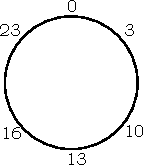
\includegraphics{images/illustrations/modular.pdf}
\end{center}

To reduce a given number using modulo 26 we can use the following function:

\[
 f(x) = x - \left\lfloor{\frac{x}{26}}\right\rfloor \times 26
\]

This says that to obtain the value of a number $x$ using modulo 26 we first divide $x$ by 26 and round down, which gives us the number of times we went around the circle. We then multiply this result by 26 again and subtract this from $x$. The final result is the remainder left over and will always be a value between 0 and 25. 

As an example, the number 28 in modulo 26 is equal to 2:
\[
	f(28) = 28 - \left\lfloor{\frac{28}{26}}\right\rfloor \times 26 = 28 - 1 \times 26 = 2
\]

The program at the end of this chapter makes use of this formula by defining a corresponding function at line 30:

\begin{screenoutput}
DEF FN F(X)=X-INT(X/26)*26
\end{screenoutput}

{\bf ROT13:} When we encrypt each plaintext letter we move forward 13 places. So the plaintext letter A becomes the ciphertext letter N, B becomes O, with latter letters "wrapping around" back to the beginning of the alphabet. Thus, the plaintext letter Z becomes the ciphertext letter M. This covers encryption. To decrypt each ciphertext letter we simply repeat the process by moving forward 13 places again, which brings us full circle, back to where we started. Thus, a ciphertext letter N becomes the plaintext letter A. 

We can see this visually as a mapping in the form of a table:

\Large
\begin{center}
  \begin{tabular}{|c|c|c|c|c|c|c|c|c|c|c|c|c|c|}
  \hline
    English Plaintext & A & B & C & D & E & F & G & H & I & J & K & L & M \\ \hline
	ROT13 Ciphertext & N & O & P & Q & R & S & T & U & V & W & X & Y & Z \\ \hline
  \end{tabular}
\end{center}

\begin{center}
  \begin{tabular}{|c|c|c|c|c|c|c|c|c|c|c|c|c|c|}
  \hline
    English Plaintext & N & O & P & Q & R & S & T & U & V & W & X & Y & Z \\ \hline
	ROT13 Ciphertext & A & B & C & D & E & F & G & H & I & J & K & L & M \\ \hline
  \end{tabular}
\end{center}

\normalsize

To encrypt using ROT13, find the plaintext letter in the top row and move down to the bottom row to find the corresponding ciphertext letter. To decrypt using ROT13, find the ciphertext letter in the bottom row and move up to the top row to find the corresponding plaintext letter.

If we consider the ROT13 cipher from a mathematical standpoint, we can see that to both encrypt and decrypt we simply add 13 to the numerical value of a plaintext or ciphertext letter and reduce it using modulo 26. This gives us a new number between 0 and 25 which corresponds to the encrypted or decrypted letter. Function $E_{ROT13}$ is the encryption function. It accepts the value of a plaintext letter $x$ as an argument and returns the value of the ciphertext letter as a result. Function $D_{ROT13}$ is the decryption function. It accepts the value of a ciphertext letter $x$ as an argument and returns the value of the plaintext letter as a result. 

\[
  E_{ROT13}(x) = (x + 13) \bmod 26
\]

\[
  D_{ROT13}(x) = (x + 13) \bmod 26
\]

Notice that the definitions of both the encryption and decryption functions are, in this case, exactly the same. 

{\bf Atbash:} Atbash is an ancient technique used to encrypt the 22-letter Hebrew alphabet, but we can apply the same logic to encrypt the 26-letter English alphabet. To encrypt a letter using Atbash we need to consider the English alphabet written backwards. So encrypting the plaintext letter A becomes the ciphertext letter Z, B becomes Y, C becomes X and so on. Decrypting the ciphertext works the same way: the ciphertext letter A becomes the plaintext letter Z, B becomes Y, C becomes X and so on.

We can see this visually as a mapping in the form of a table:

\Large
\begin{center}
  \begin{tabular}{|c|c|c|c|c|c|c|c|c|c|c|c|c|c|}
  \hline
    English Plaintext & A & B & C & D & E & F & G & H & I & J & K & L & M \\ \hline
	Atbash Ciphertext & Z & Y & X & W & V & U & T & S & R & Q & P & O & N \\ \hline
  \end{tabular}
\end{center}

\begin{center}
  \begin{tabular}{|c|c|c|c|c|c|c|c|c|c|c|c|c|c|}
  \hline
    English Plaintext & N & O & P & Q & R & S & T & U & V & W & X & Y & Z \\ \hline
    Atbash Ciphertext & M & L & K & J & I & H & G & F & E & D & C & B & A \\ \hline
  \end{tabular}
\end{center}

\normalsize

To encrypt using Atbash, find the plaintext letter in the top row and move down to the bottom row to find the corresponding ciphertext letter. To decrypt using Atbash, find the ciphertext letter in the bottom row and move up to the top row to find the corresponding plaintext letter.

If we consider the Atbash cipher from a mathematical standpoint, we can see that to encrypt and decrypt, we need to multiply by 25 and then add 25 to the numerical value of the plaintext or ciphertext and reduce it using modulo 26. This gives us a new number between 0 and 25 which corresponds to the encrypted or decrypted letter. Function $E_{Atbash}$ is the encryption function. It accepts the value of a plaintext letter $x$ as an argument and returns the value of the ciphertext letter as a result. Function $D_{Atbash}$ is the decryption function. It accepts the value of a ciphertext letter $x$ as an argument and returns the value of the plaintext letter as a result. 

\[
  E_{Atbash}(x) = (25 \times x + 25) \bmod 26
\]

\[
  D_{Atbash}(x) = (25 \times x + 25) \bmod 26
\]

Notice that the definitions of both the encryption and decryption functions are, in this case, exactly the same. 

{\bf Caesar:} The Caesar cipher is also an ancient technique used encrypt and decrypt messages. To encrypt a letter using the Caesar cipher we move three positions forward. So encrypting the plaintext letter A becomes the ciphertext letter D, B becomes E, C becomes F and so on. Decrypting the ciphertext works the opposite way. Instead of moving forward, we move three positions backward. The ciphertext letter A becomes the plaintext letter X, B becomes Y, C becomes Z and so on.

We can see this visually as a mapping in the form of a table:

\Large
\begin{center}
  \begin{tabular}{|c|c|c|c|c|c|c|c|c|c|c|c|c|c|}
  \hline
    English Plaintext & A & B & C & D & E & F & G & H & I & J & K & L & M \\ \hline
	Caesar Ciphertext & D & E & F & G & H & I & J & K & L & M & N & O & P \\ \hline
  \end{tabular}
\end{center}

\begin{center}
  \begin{tabular}{|c|c|c|c|c|c|c|c|c|c|c|c|c|c|}
  \hline
    English Plaintext & N & O & P & Q & R & S & T & U & V & W & X & Y & Z \\ \hline
    Caesar Ciphertext & Q & R & S & T & U & V & W & X & Y & Z & A & B & C \\ \hline
  \end{tabular}
\end{center}

\normalsize

To encrypt using the Caesar cipher, find the plaintext letter in the top row and move down to the bottom row to find the corresponding ciphertext letter. To decrypt using the Caesar cipher, find the ciphertext letter in the bottom row and move up to the top row to find the corresponding plaintext letter.

If we consider the Casear cipher from a mathematical standpoint, we can see that to encrypt, we need to add 3 to the numerical value of the plaintext and reduce it using modulo 26. This gives us a new number between 0 and 25 which corresponds to the encrypted letter. To decrypt, we need to subtract 3 from the numerical value of the ciphertext and reduce it modulo 26. This gives us a new number between 0 and 25 which corresponds to the decrypted letter.

Function $E_{Caesar}$ is the encryption function. It accepts the value of a plaintext letter $x$ as an argument and returns the value of the ciphertext letter as a result. Function $D_{Caesar}$ is the decryption function. It accepts the value of a ciphertext letter $x$ as an argument and returns the value of the plaintext letter as a result. 

\[
  E_{Caesar}(x) = (x + 3) \bmod 26
\]

\[
  D_{Caesar}(x) = (x - 3) \bmod 26
\]

Notice that the definitions of both the encryption and decryption functions are, in this case, different. 

We can generalise all three of the above methods by stating that they use the following encryption and decryption functions:

\[
 E(x) = (A_{1}x + B_{1}) \bmod 26
\]

\[
 D(x) = (A_{2}x + B_{2}) \bmod 26
\] 

Here, $A_{1}$, $A_{2}$, $B_{1}$ and $B_{2}$ are constants and put together they comprise the {\it encryption key} for an affine cipher.

Running the following program displays a text menu. The user can choose to encrypt or decrypt a string, or quit the program. You can practice typing in a plaintext phrase to encrypt and then decrypt the ciphertext phrase to retrieve the orginal plaintext. 

A good sample text string for testing a cipher is:

\texttt{\bf THE QUICK BROWN FOX JUMPS OVER THE LAZY DOG}

This text string, which is 43 characters long, contains 8 spaces and 35 alphabetic characters. Every character of the alphabet occurs at least once in this string, so encrypting and decrypting with it checks that every letter is transformed as expected.

Encrypting the above text string using the ROT13 cipher yields:

\texttt{\bf GUR DHVPX OEBJA SBK WHZCF BIRE GUR YNML QBT}

Encrypting the above text string using the Atbash cipher yields:

\texttt{\bf GSV JFRXP YILDM ULC QFNKH LEVI GSV OZAB WLT}

Encrypting the above text string using the Caesar cipher yields:

\texttt{\bf WKH TXLFN EURZQ IRA MXPSV RYHU WKH ODCB GRJ}

\begin{screenoutput}
10 REM *** CRYPTOGRAPHY ***
20 POKE 0,65: PRINT CHR$(142): PRINT CHR$(147)
30 DEF FN F(X)=X-INT(X/26)*26
40 C$="": P$=""
50 PRINT "SELECT AN OPTION (E, D OR Q):": PRINT
60 PRINT "{SPACE*3}[E] ENCRYPT PLAINTEXT": PRINT
70 PRINT "{SPACE*3}[D] DECRYPT CIPHERTEXT": PRINT
80 PRINT "{SPACE*3}[Q] QUIT": PRINT
90 GET S$
100 IF (S$="Q") THEN END
110 IF (S$="E") THEN GOSUB 150: GOTO 40
120 IF (S$="D") THEN GOSUB 270: GOTO 40
130 GOTO 90
140 REM ENCRYPT
150 INPUT "ENTER PLAINTEXT MESSAGE TO ENCRYPT: ", P$
160 IF P$="" THEN GOTO 150
170 M$=P$: GOSUB 390
180 IF (V=0) THEN GOSUB 460: GOTO 150
190 A=1:B=3
200 FOR I=1 TO LEN(P$)
210 :   L$ = MID$(P$,I,1)
220 :   IF (L$=" ") THEN C$=C$+" ": ELSE C$=C$+CHR$(65+(FN F(A*(ASC(L$)-65)+B)))
230 NEXT I
240 PRINT: PRINT "{REVERSE ON}ENCRYPTED CIPHERTEXT:{REVERSE OFF}", C$: PRINT
250 RETURN
260 REM DECRYPT
270 INPUT "ENTER CIPHERTEXT MESSAGE TO DECRYPT: ", C$
280 IF C$="" THEN GOTO 270
290 M$=C$: GOSUB 390
300 IF (V=0) THEN GOSUB 460: GOTO 270
310 A=1: B=-3
320 FOR I=1 TO LEN(C$)
330 :   L$ = MID$(C$,I,1)
340 :   IF (L$=" ") THEN P$=P$+" ": ELSE P$=P$+CHR$(65+(FN F(A*(ASC(L$)-65)+B)))
350 NEXT I
360 PRINT: PRINT "{REVERSE ON}DECRYPTED PLAINTEXT:{REVERSE OFF}", P$: PRINT
370 RETURN
380 REM VALIDATE
390 V = 1
400 FOR I=1 TO LEN(M$)
410 :   L$ = MID$(M$,I,1)
420 :   IF NOT (((L$ >= "A") AND (L$ <= "Z")) OR (L$=" ")) THEN V = 0
430 NEXT I
440 RETURN
450 REM ERROR MESSAGE
460 PRINT: PRINT "USE LETTERS AND SPACES ONLY": PRINT
470 RETURN	
\end{screenoutput}

If you wish to use the ROT13 cipher ensure that the following lines are changed:
\begin{screenoutput}
190 A=1: B=13
310 A=1: B=13
\end{screenoutput}

If you wish to use the Atbash cipher ensure that the following lines are changed:
\begin{screenoutput}
190 A=25: B=25
310 A=25: B=25
\end{screenoutput}

If you wish to use the Caesar cipher ensure that the following lines are changed:
\begin{screenoutput}
190 A=1: B=3
310 A=1: B=-3
\end{screenoutput}

The program listing, as written, uses the Caesar cipher by default.
